%%% LaTeX Template: Article/Thesis/etc. with colored headings and special fonts
%%%
%%% Source: http://www.howtotex.com/
%%% Feel free to distribute this template, but please keep to referal to http://www.howtotex.com/ here.
%%% February 2011
%%%
%%% Last updated September 2018 by CDM

%%%  Preamble
\documentclass[11pt,letterpaper]{article}
\usepackage[margin=1.0in]{geometry}
\usepackage[T1]{fontenc}
\usepackage[bitstream-charter]{mathdesign}
\usepackage[latin1]{inputenc}					
\usepackage{amsmath}						
\usepackage{xcolor}
\usepackage{cite}
\usepackage{hyphenat}
\usepackage{graphicx}
\usepackage{float}
\usepackage{subfigure}
\usepackage{sectsty}
\usepackage[compact]{titlesec} 
\usepackage[tablegrid]{vhistory}
\allsectionsfont{\color{accentcolor}\scshape\selectfont}

%%% Definitions
\definecolor{accentcolor}{rgb}{0.0,0.0,0.5} 
\newcommand{\teamname}{Sound Squad}
\newcommand{\productname}{Product Name}
\newcommand{\coursename}{CSE 4316: Senior Design I}
\newcommand{\semester}{Fall 2018}
\newcommand{\docname}{Project Charter}
\newcommand{\department}{Department of Computer Science \& Engineering}
\newcommand{\university}{The University of Texas at Arlington}
\newcommand{\authors}{Sochima Omenkeukwu \\ Ugo Okoye \\ Jeovanni Santos \\ Anena Sims \\ Connor Twohey}

%%% Headers and footers
\usepackage{fancyhdr}
	\pagestyle{fancy}						% Enabling the custom headers/footers
\usepackage{lastpage}	
	% Header (empty)
	\lhead{}
	\chead{}
	\rhead{}
	% Footer
	\lfoot{\footnotesize \teamname \ - \semester}
	\cfoot{}
	\rfoot{\footnotesize page \thepage\ of \pageref{LastPage}}	% "Page 1 of 2"
	\renewcommand{\headrulewidth}{0.0pt}
	\renewcommand{\footrulewidth}{0.4pt}

%%% Change the abstract environment
\usepackage[runin]{abstract}			% runin option for a run-in title
%\setlength\absleftindent{30pt}			% left margin
%\setlength\absrightindent{30pt}		% right margin
\abslabeldelim{\quad}	
\setlength{\abstitleskip}{-10pt}
\renewcommand{\abstractname}{}
\renewcommand{\abstracttextfont}{\color{accentcolor} \small \slshape}	% slanted text

%%% Start of the document
\begin{document}

%%% Cover sheet
{\centering \huge \color{accentcolor} \sc \textbf{\department \\ \university} \par}
\vspace{1 in}
{\centering \huge \color{accentcolor} \sc \textbf{\docname \\ \coursename \\ \semester} \par}
\vspace{0.5 in}
\begin{figure}[h!]
	\centering
   	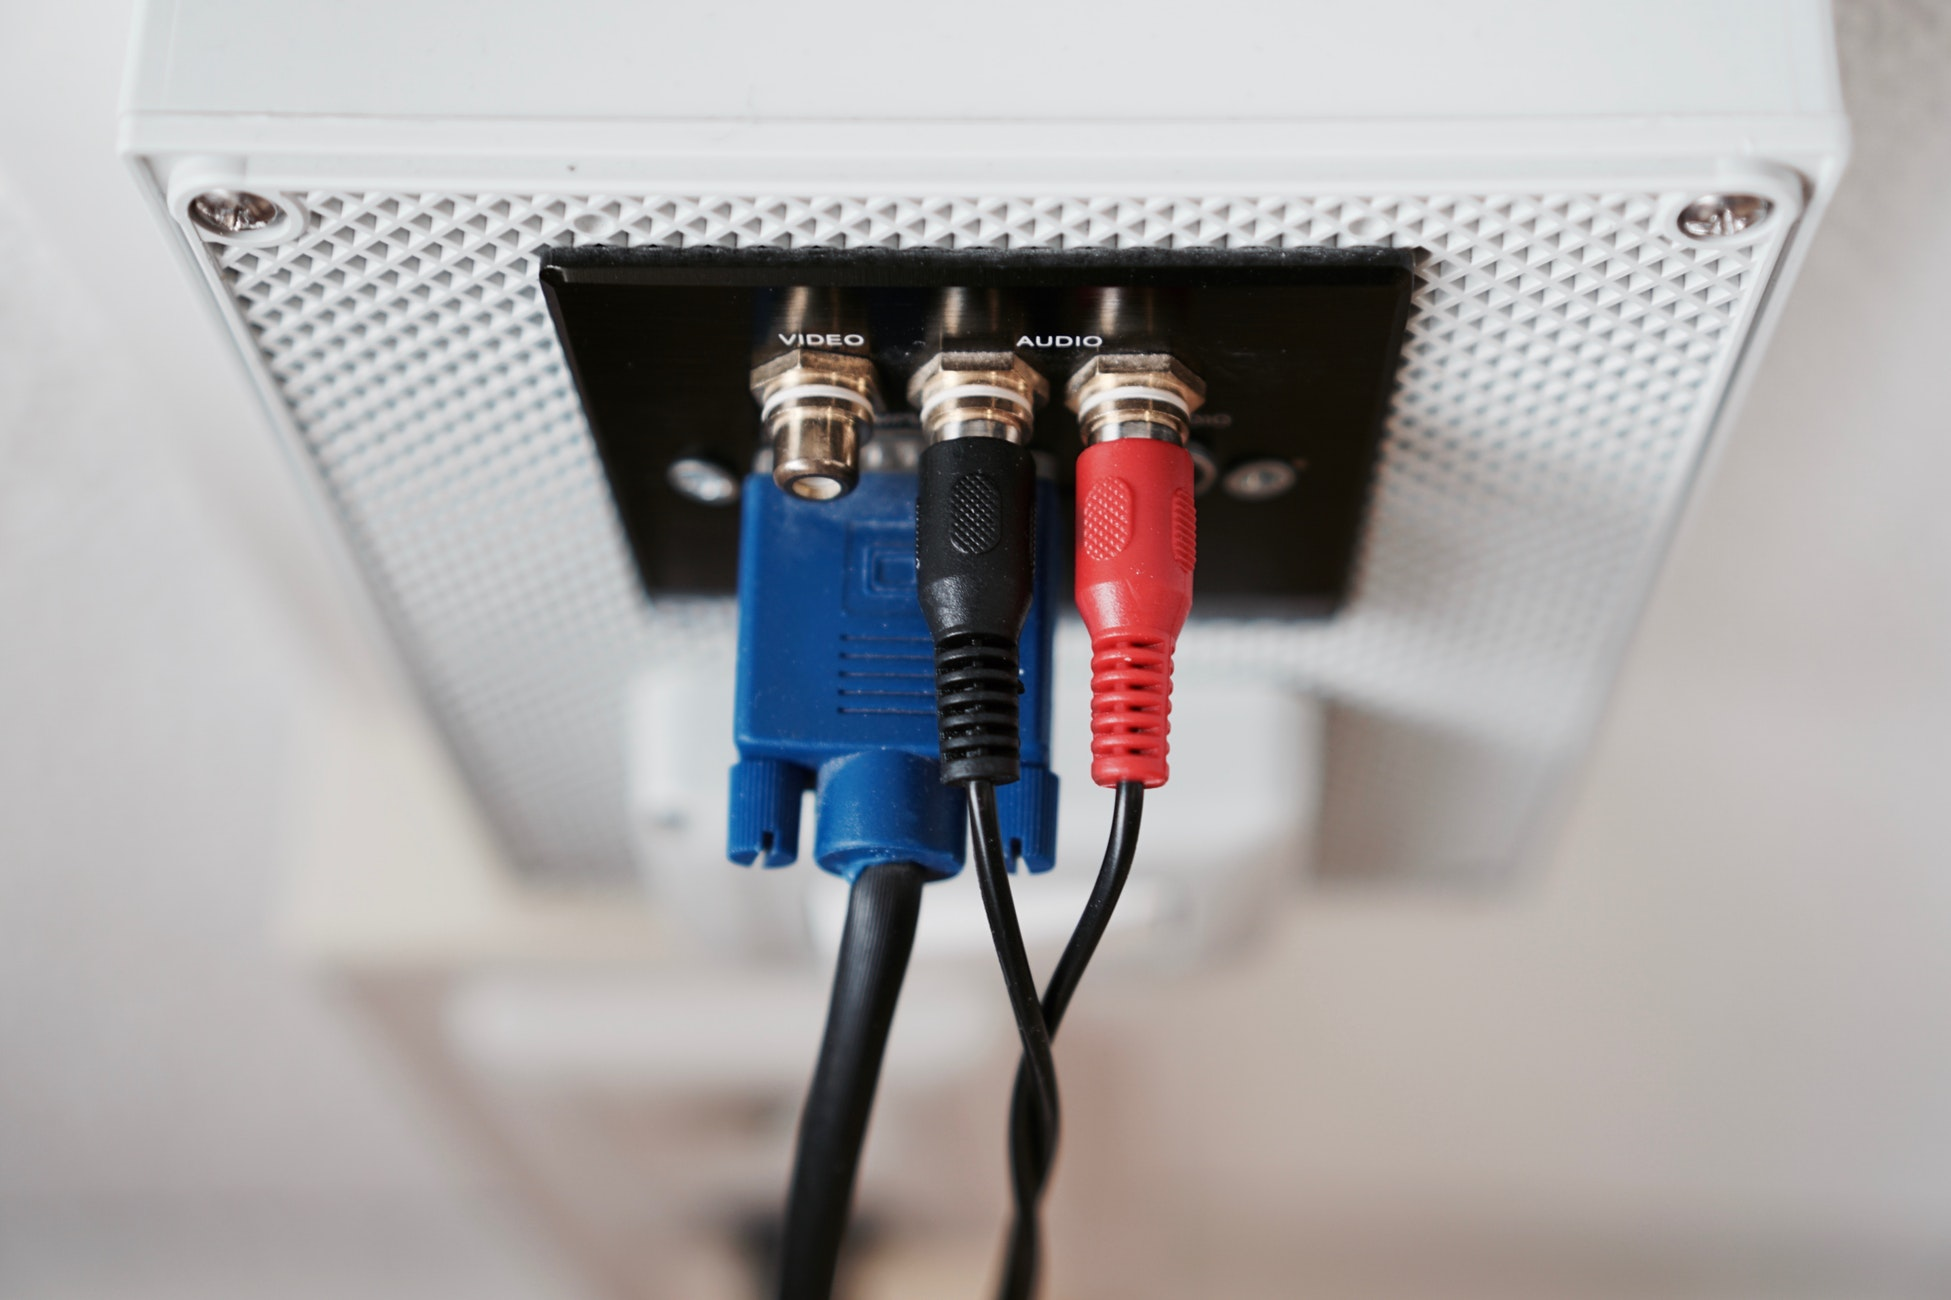
\includegraphics[width=0.60\textwidth]{images/project_charter_photo}
\end{figure}
\vspace{0.5 in}
{\centering \huge \color{accentcolor} \sc \textbf{\teamname \\ \productname} \par}
\vspace{0.5 in}
{\centering \large \sc \textbf{\authors} \par}
\newpage


%\vspace{1 in}
%\centerline{January 13th, 2012}
%\newpage

%%% Revision History
\begin{versionhistory}
  	\vhEntry{0.1}{10.01.2018}{GH}{document creation}
  	\vhEntry{0.2}{10.05.2018}{AT|GH}{complete draft}
  	\vhEntry{0.3}{10.12.2018}{AT|GH}{release candidate 1}
  	\vhEntry{1.0}{10.20.2018}{AT|GH|CB}{official release}
  	\vhEntry{1.1}{10.31.2018}{AL}{added customer change requests}
\end{versionhistory}
\newpage

%%% Table of contents
\tableofcontents
\newpage

%%% List of figures and tables (optional)
\listoffigures
%\listoftables
\newpage
\setcounter{table}{0}

%%% Agile project charter sections
\section{Vision}
We envision a world where children, youth, and adults with disabilities have the resources to be able to feel and enjoy music.


\section{Mission}
To realize this vision, we are developing an innovative vest which offers all people with disabilities the opportunity to experience music on a new level.
\section{Success Criteria}
\\
\\	
Upon completion of the prototype system, we expect the following success indicators to be observed by customers using the vest:
\begin{itemize}
  \item Increase in customer music experience 
  \item 5\% Traffic increased to Spotify 
  \item 10\% reduction in performance errors by musicians with hearing deficiency
\end{itemize}

Within 6 months after the prototype delivery date, we expect the following success indicators to be observed:
\begin{itemize}
  \item An additional 5\% reduction in performance errors by musicians with hearing deficiency
  \item Expand sales opportunities to include custom products
  \item Expanded selection of music providers
\end{itemize}

Within 12 months after the prototype delivery date, we expect the following success indicators to be observed:
\begin{itemize}
  \item Expanded product variation, including different sizes, wristbands, and higher quality vests
  \item Additional settings for the vest model 
  \item 10\% increase in product sales
\end{itemize}



\newpage

%%% Remaining project charter sections
\section{Background}
An in-depth explanation of the problem, including the "business case". What is wrong with the status-quo that justifies undertaking this project? If you have a clear customer or sponsor, why do they want you to work on this? This section should occupy 1/2 - 1 full page.
\section{Related Work}
Discuss the state-of-the-art with respect to your product. What solutions currently exist, and in what form (academic research, enthusiast prototype, commercially available, etc)? Include references and citations as necessary \cite{Rubin2012}. If there are existing solutions, why won't they work for your customer (too expensive, not fast enough, not reliable enough, etc.). This section should occupy 1/2 - 1 full page, and should include at least 5 references to related work.
\section{System Overview}
Product will be a vest, custom made, from a light weight material. The vest will be one size fits all, with adjustable straps for comfort. Several haptic motor controllers will be strategically sewn into the chest of the vest, along with a micro-controller and button control panel. The motors will vibrate within the vest according to the tempo of music played by the user. The music will be supplied and transmitted to the vest through Spotify API calls. The user will be able to log into the vest’s web based application to select music to play through the vest. The music will play in audio through the device accessing the web app, as well as vibrate through the vest. Profile settings and advanced vest settings can be set in the vest’s web application. The button controls on the vest will allow the customer to make local changes to the function of the vest, like vibration intensity. The vest will receive sound waves and instructions for the motors from a raspberry pi micro controller. The micro-controller will filter through sound waves and send instruction to the motors.
\section{Roles \& Responsibilities}
Who are the stakeholders of the project? Who will be the point of contact from the sponsor or customer side? Who are the team members, and what will be their areas of responsibility? Will your team maintain the product owner and scrum master for the whole project, or will that role change periodically? This section should occupy 1/2 - 1 full page.
\section{Cost Proposal}
The approximate budget for this project will be $800 will be funded by UTA CSE Department.

\subsection{Preliminary Budget}

\begin{table}[h]
\resizebox{\textwidth}{!}{
\begin{tabular}{|l|l|}
\hline
 \textbf{Items} & \textbf{Costs}} \\ \hline
 Bass Shaker  & $20 a unit - $100 a unit \\ \hline
 Vest  & $20 - $100 \\ \hline
 Raspberry Pi  & $40\\ \hline
\end{tabular}}
\caption{Preliminary budget} 
\end{table}


\subsection{Current \& Pending Support}
There is a funding support of $800 coming from the UTA CSE Department.

\section{Facilities \& Equipment}
The Lab room in the Engineering Research building will be needed to work on the functional part of the vest, which comprises of the raspberry pi, and the additional components needed for the vest. Other work areas like the Fab lab might be used to work on the making the vest itself. Currently the complete list of equipment needed have not been completely decided on, but we will be using a raspberry pi, and the materials which will be used to make the vest. There is not necessarily any space for the demo, as it would be worn by an individual, so the classroom where the demo will take place is sufficient. To make to vest, there is a possibility that the services of the Theater students will be needed. 

\section{Assumptions}

\begin{itemize}
  \item The vest can be tested anywhere as it has to be worn by an individual to be useful
  \item The raspberry pi would be put at the bottom of the vest which will be padded in the event that it heats up 
  \item The vest will be made of a light material in order not to be too heavy for the user
  \item There will be a website which will serve as a user interface in order to interact with the vest. There would also be dials on the vest that the user can use to change the sound volume.
  \item The total cost of the vest will not exceed 800 dollars
  \item Work on the vest will begin in this first semester.
\end{itemize}

\section{Constraints}
Constraints are limitations imposed on the project, such as the limitation of cost, schedule, or resources, and you have to work within the boundaries restricted by these constraints. All projects have constraints, which are defined and identified at the beginning of the project.

Constraints are outside of your control. They are imposed upon you by your client, organization, government regulations, availability of resources, etc. Occasionally, identified constraints turn out to be false. This is often beneficial to the development team, since it removes items that could potentially affect progress.

This section should contain a list of at least 5 of the most critical constraints related to your project. For example:

The following list contains key constraints related to the implementation and testing of the project.

\begin{itemize}
  \item Final prototype demonstration must be completed by May 1st, 20XX
  \item The customer will provide no more than two maintenance personnel to assist in on-site installation
  \item Customer installation site will only be accessible by development team during normal business hours
  \item Total development costs must not exceed \$800
  \item All data obtained from customer site must be reviewed and approved for release by the Information Security Office prior to being copied to any internet connected storage medium
\end{itemize}

\section{Risks}
This section should contain a list of at least 5 of the most critical risks related to your project. Additionally, the probability of occurrence, size of loss, and risk exposure should be listed. For size of loss, express units as the number of days by which the project schedule would be delayed. For risk exposure, multiply the size of loss by the probability of occurrence to obtain the exposure in days. For example:

The following high-level risk census contains identified project risks with the highest exposure. Mitigation strategies will be discussed in future planning sessions.

\begin{table}[h]
\resizebox{\textwidth}{!}{
\begin{tabular}{|l|l|l|l|}
\hline
 \textbf{Risk description} & \textbf{Probability} & \textbf{Loss (days)} & \textbf{Exposure (days)} \\ \hline
 Bass shaker or vibration device failing  & 0.05 & 20 & 1 \\ \hline
 Testing grounds are not available  & 0.10 & 4 & 0.4 \\ \hline
 Battery Failing  & 0.05 & 5 & 0.25 \\ \hline
 Delays in shipping from overseas vendors  & 0.20 & 25 & 5 \\ \hline
 Vest design delayed by vest makers & 0.15 & 10 & 1.5 \\ \hline
\end{tabular}}
\caption{Overview of highest exposure project risks} 
\end{table}

\section{Documentation \& Reporting}
%%% In this section, you will describe all of the various artifacts that you will generate and maintain during the project life cycle. Describe the purpose of each item below, how the content will be generated, where it will be stored, how often it will be updated, etc. Replace the default text for each section with your own description. Reword this paragraph as appropriate.

\subsection{Major Documentation Deliverables}
These deliverables are major grade components of the course. Completing these documents should generally be the sprint goal during the applicable sprint period. Remove this paragraph from your draft, but leave the heading.

\subsubsection{Project Charter}
Describe how this document will be maintained and updated (how often, under what circumstances, etc.). When will the initial version be delivered? When will the final version be delivered?

\subsubsection{System Requirements Specification}
This documnet will be updated anytime a new portion is added to the project. It will also be updates if there is a portion of the system that is found faulty or not feasible to work with. The intial version will be delievered along with the first charter report while the final version will be delievered when the design of the system has been concluded on and no changes need to be made.

\subsubsection{Architectural Design Specification}
This documnet will be updated anytime a new portion is added to the project. It will also be updates if there is a portion of the system that is found faulty or not feasible to work with. The intial version will be delievered along with the first charter report while the final version will be delievered when the design of the system has been concluded on and no changes need to be made.

\subsubsection{Detailed Design Specification}
This documnet will be updated anytime a new portion is added to the project. It will also be updates if there is a portion of the system that is found faulty or not feasible to work with. The new chnages will be described in detail showing what was removed or what was added in the design. The intial version will be delievered along with the first charter report while the final version will be delievered when the design of the system has been concluded on and no changes need to be made.

\subsection{Recurring Sprint Items}
The following items will be documented and maintained during each individual sprint. Remove this paragraph from your draft, but leave the heading.

\subsubsection{Product Backlog}
Team members will meet to determine requirements and break them down into features, which will be added to the backlog. Team members will determine the priority of each feature with a group vote, giving the most weight to items that progress development. The backlog will be a Google workbook document that can be edited and tracked by all team members.

\subsubsection{Sprint Planning}
At the end of one sprint there will be a meeting to discuss the next sprint. The backlog will be updated and tasks for each feature will be assigned. There will be 4 sprints, each lasting 3 weeks.

\subsubsection{Sprint Goal}
The team as a whole will determine the end goal of each sprint during the sprint planing meeting. The professor will be consulted periodically through the process via email and in-person communication. 

\subsubsection{Sprint Backlog}
The team as a whole will determine which backlog items are implemented into a sprint and when. The backlog will be a Google workbook document that can be edited and tracked by all team members.

\subsubsection{Task Breakdown}
The team will assign tasks during the sprint planing meeting. Team members can volunteer for tasks, or tasks can be assigned based on skill set. Task will be equally distributed across all members. Each team member will be responsible for tracking and recording the time spent on their assigned tasks. 

\subsubsection{Sprint Burn Down Charts}
Team members will alternate being scrum master. The scrum master will be responsible for monitoring the backlog. The backlog will generate a burn chart based on the data input into the table. Each team member will have access to update the backlog with the amount of time spent on each task. When this value is updated the burn chart will update the graph.

\begin{figure}[h!]
    \centering
    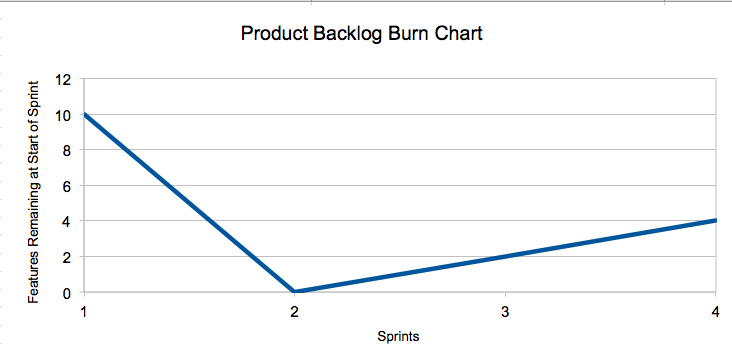
\includegraphics[width=0.5\textwidth]{images/burn_down_chart_example}
    \caption{Example sprint burn down chart}
\end{figure}

\subsubsection{Sprint Retrospective}
The sprint retrospective will take place at a team meeting. It will occur after every sprint has passed . The group will document what worked and should be maintained, what needs to improve and also resolve any conflict that arises in the just concluded sprint. It will be due about a week after the meeting has been held.

\subsubsection{Individual Status Reports}
Each member would report on any task that has been asssigned to them to work on. It will be reported anytime there is a new task assigned and also when the report needs to be turned in. Every item assigned to each individual relating to the building of the project is considered a key item and should be added in the report.

\subsubsection{Engineering Notebooks}
The engineering notebook will be updated anytime work is done on the project. Therefore each member would always enter any part of the project they are working on. The minimum amount of pages as of now should be 1 page. Every section of the project assigned by the group is considered an interval so each interval is till the that section is finished. At least two other team members will sign the engineering notebooks as witnesses for each page.

\subsection{Closeout Materials}
The following materials, in addition to major documentation deliverables, will be provided to the customer upon project closeout. Remove this paragraph from your draft, but leave the heading.

\subsubsection{System Prototype}
What will be included in the final system prototype? How and when will this be demonstrated? Will there be a Prototype Acceptance Test (PAT) with your customer? Will anything be demonstrated off-site? If so, will there be a Field Acceptance Test (FAT)?

\subsubsection{Project Poster}
What will be included on the poster, what will be the final dimensions, and when will it be delivered?

\subsubsection{Web Page}
What will be included on the project web page? Will it be accessible to the public? When will this be delivered? Will it be updated throughout the project, or just provided at closeout (at a minimum, you need to provide a simple web page at the end).

\subsubsection{Demo Video}
What will be shown in the demo video(s)? Will you include a B-reel footage for future video cuts? Approximately how long will the video(s) be, and what topics will be covered?

\subsubsection{Source Code}
How will your source code be maintained? What version control system will you adopt? Will source code be provided to the customer, or binaries only? If source code is provided, how will it be turned over to the customer? Will the project be open sourced to the general public? If so, what are the license terms (GNU, GPL, MIT, etc.). Where will the license terms be listed (in each source file, in a single readme file, etc.).

\subsubsection{Source Code Documentation}
What documentation standards will be employed? Will you use tools to generate the documentation (Doxygen, Javadocs, etc.). In what format will the final documentation be provided (PDF, browsable HTML, etc.)?

\subsubsection{Hardware Schematics}
Will you be creating printed circuit boards (PCBs) or wiring components together? If so, list each applicable schematic and what sort of data it will contain (PCB layout, wiring diagram, etc.). If your project is purely software, omit this section.

\subsubsection{CAD files}
Will the project involve any mechanical design, such as 3D printed or laser-cut parts? If so, what software will you use to generate the files and what file formats will you provide in your closeout materials (STL, STEP, OBJ, etc.). If your project is purely software, omit this section.

\subsubsection{Installation Scripts}
How will the customer deploy software to new installations? Will you provide installation scripts, install programs, or any other tools to improve the process? Will there be multiple scripts provided (perhaps separate scripts for the graphical front end and back end server software)? 

\subsubsection{User Manual}
Will you customer need a printed or digital user manual? Will they need a setup video? Decide now what will be provided and discuss.

\newpage

%%% References
\bibliographystyle{plain}
\bibliographystyle{reference/IEEEtran_custom}
\bibliography{reference/refs}{}

\end{document}